%
% potenzverteilung.tex -- Abschnitt ueber Pareto-Verteilung im Kapitel 5
%
% (c) 2015 Prof Dr Andreas Mueller, Hochschule Rapperswil
%
\subsection{Potenzgesetze} \label{potenzgesetze}
% XXX neues Beispiel: Verteilung der Partikelgrössen in Planetenringen
%     http://www.pnas.org/content/112/31/9536
%     Size distribution of particles in Saturn's rings from aggregation
%     and fragmentation
%     Nikolai Brilliantova, P. L. Krapivskyb, Anna Bodrovac,d, Frank Spahnd,
%     Hisao Hayakawae, Vladimir Stadnichukc, and Jürgen Schmidtf,1
%     Proceedings of the National Academy of Sciences of the USA
%     vol 112(31), 2015, pp 9536-9541
%
Die Normalverteilung beschreibt physikalische Grössen sehr erfolgreich,
die vor allem in einer bestimmten Grösse vorkommen.
Menschen sind zum
Beispiel im Durchschnitt etwa 1.80m gross, Abweichungen kommen vor, sind
aber sehr selten, 5m grosse Menschen gibt es nicht.


Andererseits gibt es auch Grössen, die einen weiten Bereich von möglichen
Werten annehmen.
Mondkrater können mehrere Kilometer gross sein, oder auch
nur ein paar Millimeter.
Der Entstehungsmechanismus ist unabhängig von der
Grössenskala immer der Selbe.
Diese Unabhängigkeit von der Grössenskala
sollte sich auch in der Verteilungsfunktion der Grösse niederschlagen.
In diesem Abschnitt sollen die Eigenschaften solcher Verteilungen abgeleitet
werden.

\subsubsection{Skalenunabhängigkeit und Potenzgesetze}
Wir untersuchen nun Zufallsvariablen $X$, wie zum Beispiel den Durchmesser
von Mondkratern. 
Die Verteilung soll also für jeden beliebigen
Mass\-stab gelten.
Die Form des Graphen von $\varphi(x)$ darf sich nicht ändern,
wenn wir zu einer anderen Skala übergehen.
Für jede Zahl $b>0$ muss es also eine Konstante $g(b)$ geben, 
so dass
\[
\varphi(bx)=g(b)\varphi(x).
\]
Leitet man dies nach $b$ ab und setzt $b=1$, erhält man
\begin{align*}
x\varphi'(x)&=g'(1)\varphi(x).
\end{align*}
Dies ist eine gewöhnliche lineare Differentialgleichung
erster Ordnung, die man mit Separation der Variablen
lösen kann
\begin{align*}
\frac{\varphi'(x)}{\varphi(x)}&=g'(1)\frac1x
\\
\int\frac{\varphi'(x)}{\varphi(x)}\,dx&=g'(1)\int\frac{dx}x + c
\\
\log \varphi(x)&=g'(1)\log x+c
\\
\varphi(x)&=Cx^{-\alpha}\qquad\text{mit $\alpha=-g'(1)$}.
\end{align*}
Der Exponent $-\alpha$ ist immer negativ, also $\alpha > 0$,
da $g'(1)<0$ sein muss.

\begin{definition}
Eine Verteilung mit der Dichtefunktion
\[
\varphi(x)=\begin{cases}
Cx^{-\alpha}&\qquad x>x_{\min}\\
0&\qquad\text{sonst}
\end{cases}
\]
heisst Potenzgesetz oder Pareto-Verteilung.
\end{definition}
Damit dies eine Wahrscheinlichkeitsverteilung definiert, muss $C$
so gewählt werden, dass das Integral über $\mathbb R$ den Wert $1$
ergibt,
\begin{align*}
1=\int_{-\infty}^\infty\varphi(x)\,dx
&=
\int_{x_{\min}}^\infty Cx^{-\alpha}\,dx
\\
&=
\left[-\frac{C}{1-\alpha}x^{1-\alpha}\right]_{x_{\min}}^\infty
\\
&=
C\frac{x_{\min}^{1-\alpha}}{\alpha-1}
\\
\Rightarrow\qquad
C
&=
\frac{\alpha-1}{x_{\min}^{1-\alpha}}.
\end{align*}
Die Berechnung der Normierungskonstanten zeigt auch, dass die Normierung
für $\alpha \le 1$ nicht mehr möglich ist, Potenzgesetze sind daher
nur für $\alpha > 1$ möglich.

\begin{satz}
Die Dichtefunktion einer nach einem Potenzgesetz verteilten Zufallsvariablen
ist 
\[
\varphi(x)=\begin{cases}
\displaystyle
\frac{\alpha-1}{x_{\min}^{1-\alpha}}
x^{-\alpha}&\qquad x>x_{\min}
\\
0&\qquad\text{sonst},
\end{cases}
\]
wobei $\alpha>1$ gelten muss.
\end{satz}
\begin{figure}
\centering
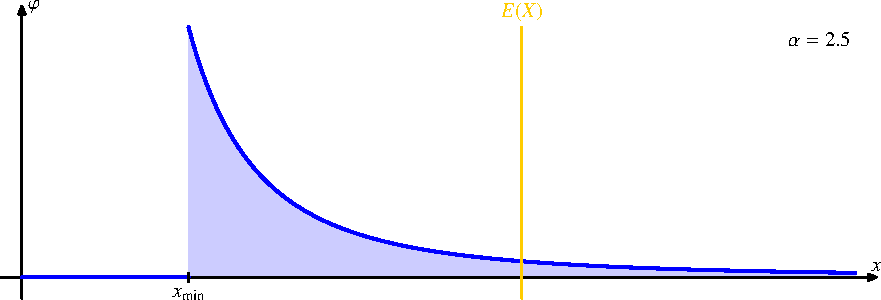
\includegraphics{images/power-2.pdf}
\caption{Wahrscheinlichkeitsdichte einer Potenzverteilung mit $\alpha=2.5$,
diese Verteilung hat keine Varianz
\label{pareto-verteilung-2.5}}
\end{figure}
\begin{figure}
\centering
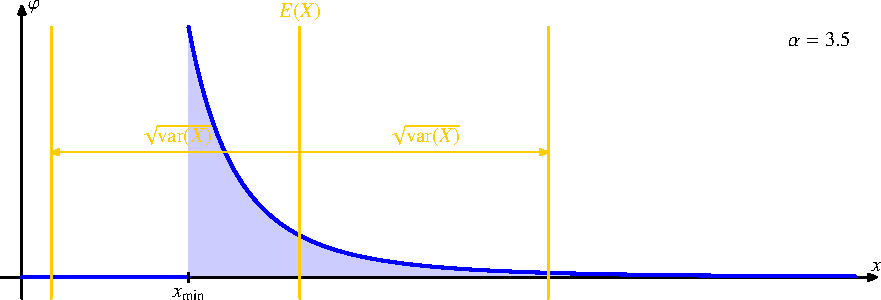
\includegraphics{images/power-3.pdf}
\caption{Wahrscheinlichkeitsdichte einer Potenzverteilung mit $\alpha=3.5$
\label{pareto-verteilung-3.5}}
\end{figure}

Nach einem Potenzgesetz verteilte Zufallsvariablen kann man daran
erkennen, dass die Dichtefunktion in einer doppelt logarithmischen
Darstellung eine Gerade ist.
Wegen
\[
\log p(x)=-\alpha \log x+\log C
\]
ist die Steigung der Geraden $-\alpha$.

\subsubsection{Erwartungswert und Varianz}
Mit Hilfe der Dichtefunktion können die üblichen Kennzahlen der Verteilung
berechnet werden.
Der Erwartungswert einer nach einem Potenzgesetz verteilten Zufallsvariable $X$
ist
\begin{align*}
E(X)&=
\int_{-\infty}^\infty x\varphi(x)\,dx
\\
&=
\int_{x_{\min}}^\infty 
x
\frac{\alpha-1}{x_{\min}^{1-\alpha}}
x^{-\alpha}\,dx
\\
&=
\frac{\alpha-1}{x_{\min}^{1-\alpha}}
\left[\frac{1}{2-\alpha}x^{2-\alpha}\right]_{x_{\min}}^\infty
\\
&=
\frac{\alpha-1}{\alpha-2}x_{\min}.
\end{align*}
Dies ist natürlich nur möglich, solange $\alpha > 2$.

Für die Varianz berechnet man zunächst das zweite Moment
\begin{align*}
E(X^2)&=
\int_{-\infty}^\infty x^2\varphi(x)\,dx
\\
&=
\int_{x_{\min}}^\infty 
x^2
\frac{\alpha-1}{x_{\min}^{1-\alpha}}
x^{-\alpha}\,dx
\\
&=
\frac{\alpha-1}{\alpha-1}\frac1{x_{\min}^{1-\alpha}}\left[-x^{3-\alpha}\right]_{x_{\min}}^\infty
\\
&=
\frac{\alpha-1}{\alpha-3}x_{\min}^2.
\end{align*}
Dieses Moment existiert also nur, wenn $\alpha >3$.
Die Varianz wird damit
\begin{align*}
\operatorname{var}(X)
&=
E(X^2)-E(X)^2
\\
&=
\biggl(
\frac{\alpha-1}{\alpha-3}-\biggl(\frac{\alpha-1}{\alpha-2}\biggr)^2
\biggr)x_{\min}^2.
\end{align*}
\begin{satz}
Ist $X$ verteilt nach einem Potenzgesetz mit Exponent $\alpha$, dann
existiert für $\alpha>2$ ein Erwartungswert
\[
E(X)
=
\frac{\alpha-1}{\alpha-2}x_{\min}
\]
und für $\alpha >3$ auch eine Varianz
\[
\operatorname{var}(X)
=
\biggl(
\frac{\alpha-1}{\alpha-3}-\biggl(\frac{\alpha-1}{\alpha-2}\biggr)^2
\biggr)x_{\min}^2.
\]
\end{satz}

\subsubsection{Median} \label{subsubsection-median}
Der Median ist derjenige Wert $x_{\frac12}$ der Zufallsvariablen,
für den die Verteilungsfunktion den Wert $\frac12$ annimmt, also
\begin{align*}
\frac12=\int_{-\infty}^{x_{\frac12}}\varphi(x)\,dx
&=
\int_{x_{\min}}^{x_{\frac12}}
\frac{\alpha-1}{x_{\min}^{1-\alpha}}
x^{-\alpha}\,dx
\\
&=
\frac{\alpha-1}{x_{\min}^{1-\alpha}}\left[
\frac{x^{1-\alpha}}{1-\alpha}
\right]_{x_{\min}}^{x_{\frac12}}
\\
&=
\frac{x_{\min}^{1-\alpha}-x_{\frac12}^{1-\alpha}}{x_{\min}^{1-\alpha}}
\\
&=
1-\left(
\frac{x_{\frac12}}{x_{\min}}
\right)^{1-\alpha}.
\end{align*}
Diese Gleichung kann man nach $x_{\frac12}$ auflösen:
\begin{align*}
\frac{x_{\frac12}}{x_{\min}}
&=
\left(\frac12\right)^{\frac1{1-\alpha}}
\\
x_{\frac12}&=2^{\frac1{\alpha-1}}x_{\min}.
\end{align*}
\begin{satz}
Ist die Zufallsvariable $X$ nach einem Potenzgesetz mit Exponent $\alpha>1$
verteilt, existiert der Median
\[
x_{\frac12}=2^{\frac1{\alpha-1}}x_{\min}.
\]
\end{satz}
\begin{table}
\renewcommand{\arraystretch}{2}
\begin{center}
\begin{tabular}{|l|l|}
\hline
Name&Potenzverteilung, Pareto-Verteilung\\
\hline
Dichtefunktion&
\begin{minipage}{3.7in}
\vskip5pt
$\displaystyle
\begin{cases}
\frac{\alpha-1}{x_{\min}}\biggl(\frac{x}{x_{\text{min}}}\biggr)^{-\alpha}&\qquad x>x_{\text{min}}\\
0&\qquad\text{sonst}
\end{cases}
$
\end{minipage}
\\[15pt]
Verteilungsfunktion&
\begin{minipage}{3.7in}
\vskip3pt
$\displaystyle
\begin{cases}
1-\biggl(\frac{x}{x_{\text{min}}}\biggr)^{1-\alpha}&\qquad x>x_{\text{min}}\\
0&\qquad\text{sonst}
\end{cases} $
\end{minipage}
\\
Erwartungswert&$\displaystyle\frac{\alpha-1}{\alpha-2}x_{\text{min}}$,
undefiniert für $\alpha\le 2$\\
Varianz&$\displaystyle
\biggl(
\frac{\alpha-1}{\alpha -3}-\biggl(\frac{\alpha-1}{\alpha-2}\biggr)^2
\biggr)x_{\text{min}}^2$, undefiniert für $\alpha \le 3$\\
$P(|X-E(X)|>\varepsilon)$&$\displaystyle $ \\
Median&$2^{\frac1{\alpha-1}}x_{\text{min}}$\\
\hline
Anwendungen&\begin{minipage}{3.7in}%
\vskip5pt
\strut
$\bullet$ Häufkeitsverteilung für skaleninvariante Prozesse\\
$\bullet$ Einkommensverteilung\\
$\bullet$ Grösse und Häufigkeit von Mondkratern\\
$\bullet$ Verkaufszahlen von Büchern\\
$\bullet$ Einwohnerzahlen von Städten
\strut
\end{minipage}\\[28pt]
\hline
\end{tabular}
\end{center}
\caption{Datenblatt der Potenzverteilung\label{datenblatt:potenzverteilung}}
\end{table}

\subsubsection{Die 80/20-Regel}
\begin{figure}
\begin{center}
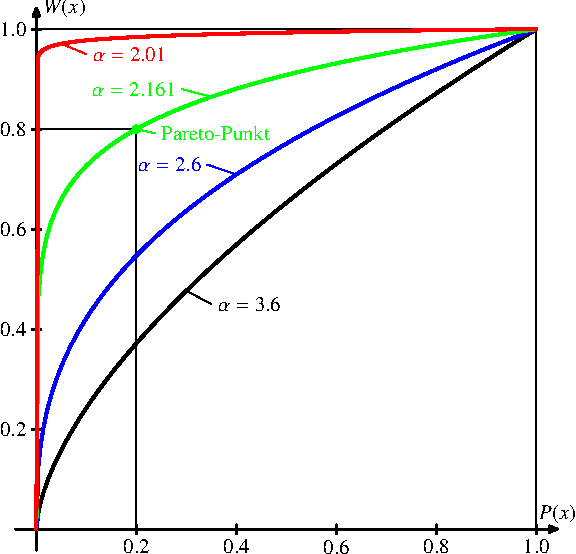
\includegraphics{images/power-4.pdf}
\end{center}
\caption{Kurven $(P(x),W(x))$ für verschiedene Werte von $\alpha$\label{wp}}
\end{figure}
Die 80/20-Regel besagt, dass 20\% der Werte für 80\% des kumulierten Wertes
verantwortlich sind.

Allgemeiner können wir für jedes $x$ nach der Wahrscheinlichkeit
eines Wertes $>x$ fragen und ihn vergleichen mit dem gesamten Erwartungswert,
den die Werte $>x$ ergeben.
Die Wahrscheinlichkeit eines Wertes $>x$ ist
\begin{align}
P(x)
&=
\int_x^\infty
\frac{\alpha-1}{x_{\min}^{1-\alpha}}
x^{-\alpha}
\,dx
\notag
\\
&=
-\frac{1}{x_{\min}^{1-\alpha}}
\left[x^{1-\alpha}\right]_x^\infty
=
\left(
\frac{x}{x_{\min}}
\right)^{1-\alpha}.
\label{px}
\end{align}
Den Beitrag der Werte $>x$ zum Erwartungswert berechnet die Funktion
\begin{equation}
W(x)=\frac%
{\int_x^\infty \xi\varphi(\xi)\,d\xi}%
{\int_{x_{\min}}^\infty \xi\varphi(\xi)\,d\xi}.
\label{wx}
\end{equation}
Nach den bisher durchgeführten Rechnungen ist
\[
W(x)=\left(\frac{x}{x_{\min}}\right)^{2-\alpha}
=P(x)^{\frac{\alpha-2}{\alpha-1}}.
\]
Die Abbildung \ref{wp} zeigt den Zusammenhang zwischen $P(x)$ und $W(x)$
für verschiedene Werte von $\alpha$

Die 80/20-Regel entspricht der Kurve, die durch den 
Punkt mit $P(x)=0.2$ und $W(x)=0.8$ geht, also
\begin{align*}
0.8&=0.2^{\frac{\alpha-2}{\alpha-1}}
\\
\frac{\log 0.8}{\log 0.2}
&=
\frac{\alpha-2}{\alpha-1}.
\end{align*}
Schreiben wir für das Verhältnis der Logarithmen auf der linken
Seite $\lambda$ ergibt sich die Gleichung
\begin{align*}
\lambda
&=
\frac{\alpha-2}{\alpha-1}
\\
\alpha(\lambda-1)&=\lambda-2
\\
\alpha&=\frac{\lambda-2}{\lambda-1}.
\end{align*}
Im konkreten Fall ist der numerische Wert für $\alpha=2.160964$.

Für $\alpha\le 2$ existieren die Erwartungswerte nicht mehr, die
Integrale in (\ref{wx}) divergieren.
Wenn man jedoch
eine gemeinsame obere Schranke $x_{\max}$ verwendet, kann man $P$
und $W$ als von dieser Schranke abhängige Grössen immer noch
definieren und den Grenzwert für $x_{\max}\to\infty$ erst nachher
durchführen.
Dabei stellt sich heraus, dass
\begin{align*}
W(x)
&=
\lim_{x_{\max}\to\infty}
\frac%
{\int_x^{x_{\max}} \xi\varphi(\xi)\,d\xi}%
{\int_{x_{\min}}^{x_{\max}} \xi\varphi(\xi)\,d\xi}.
\\
&=
\lim_{x_{\max}\to\infty}
\frac%
{x_{\max}^{2-\alpha}-x^{2-\alpha}}%
{x_{\max}^{2-\alpha}-x_{\min}^{2-\alpha}}
=1.
\end{align*}
Sobald also $\alpha\le2$ ist, sind alle Beiträge zum Erwartungswert
in einem noch so kleinen Teil der grössten Werte konzentriert.

"Ubersetzt in die aktuelle Diskussion über Vermögensverteilungen
und Managerlöhne bedeutet dies, dass für $\alpha\le2$ jeder noch so
kleine Teil der Spitze der Einkommenspyramide alles besitzt, und alle
anderen nichts.
Je näher $\alpha$ an $2$ kommt desto extremer wird
das Ungleichgewicht zwischen arm und reich.

\subsubsection{Parameter schätzen}
Um den Parameter $\alpha$ zu schätzen könnte man für die Punkte
eines Histogramms eine lineare Regression durchführen.
Eine Maximum-Likelihood-Schätzung führt jedoch direkter zum
Ziel.
Mit der Dichtefunktion
\[
\varphi(x)=\frac{\alpha-1}{x_{\min}}\left(\frac{x}{x_{\min}}\right)^{-\alpha}
\]
wird die Likelihood-Funktion
\[
L(\alpha;x_1,\dots,x_n)=
\left(\frac{\alpha-1}{x_{\min}}\right)^n
\prod_{i=1}^n
\left(\frac{x_i}{x_{\min}}\right)^{-\alpha}.
\]
$\alpha$ ist so zu bestimmen, dass $L(\alpha;x_1,\dots,x_n)$ maximal
wird.
Dies ist gleichbedeutend damit, dass der natürliche 
Logarithmus $\log L(\alpha;x_1,\dots,x_n)$ maximiert wird.
Partielle Ableitung nach $\alpha$ ergibt
\begin{align*}
\frac{\partial}{\partial \alpha}
L(\alpha;x_1,\dots,x_n)
&=
\frac{\partial}{\partial\alpha}
\biggl[
n\log(\alpha-1)-n\log x_{\min}
-\alpha\biggl( \sum_{i=1}^n\log x_i-n \log x_{\min}\biggr)
\biggr]
\\
&=
\frac{n}{\alpha-1}-\sum_{i=1}^n\log x_i-n\log x_{\min}=0.
\end{align*}
Diese Gleichung kann man nach $\alpha$ auflösen und findet
\begin{align*}
\frac{n}{\alpha-1}
&=
\sum_{i=1}^n \log\frac{x_i}{x_{\min}}
\\
\alpha&=1+\frac{n}{
\sum_{i=1}^n \log\frac{x_i}{x_{\min}}
}.
\end{align*}


